% =============================================================
%  CC-iGPT v2 答辩 beamer (精简版，10 页，图片用户自插)
%  编译: xelatex defense.tex (双编译保 TOC/目录正确)
%  Overleaf: 上传本单文件，编译器选 XeLaTeX 即可
% =============================================================
\documentclass[10pt,aspectratio=169]{beamer}
\usetheme{metropolis}

\usepackage[UTF8]{ctex}      % Overleaf 自带，中英混排
\usepackage{amsmath,amssymb}
\usepackage{booktabs}
\usepackage{tikz}
\usetikzlibrary{positioning,arrows.meta,fit,backgrounds}
\usepackage{graphicx}
\graphicspath{{../figures/}{./}}

% ── 配色（与 demo 一致）──
\definecolor{ours}{HTML}{6C8CFF}
\definecolor{accent}{HTML}{FF9800}
\definecolor{muted}{HTML}{8B8FA3}
\setbeamercolor{alerted text}{fg=accent}
\setbeamercolor{progress bar}{fg=ours}
\setbeamercolor{frametitle}{bg=ours}

% ── 占位框宏（用户后续用 \includegraphics 替换）──
% 用法: \figplaceholder{建议素材文件名}{宽}{高}
\newcommand{\figplaceholder}[3]{%
  \begin{center}
  \begin{tikzpicture}
    \draw[dashed, gray!55, line width=0.8pt]
      (0,0) rectangle (#2,#3);
    \node[align=center, gray!70] at (#2/2, #3/2)
      {\small\textit{[ 此处插入图片 ]}\\[2pt]
       \scriptsize\texttt{#1}};
  \end{tikzpicture}
  \end{center}
}

% ── 标题信息（用户填空）──
\title{基于 MDL 原则的深度图像压缩}
\subtitle{CC-iGPT 双尺度条件式自回归}
\author{[ 姓名 ]}
\institute{[ 学院 / 学校 ] \quad 指导教师: [ 导师姓名 ]}
\date{2026 年 5 月 28 日}

\begin{document}

% ============================== 1. 封面 ==============================
\maketitle

% ============================== 2. 命题 ==============================
\begin{frame}{命题：压缩即预测}
\textbf{Shannon (1948)} \;源编码定理：随机序列的最优编码长度下界为其负对数似然
\[
L^{\star}(x) \;=\; -\log_2 p(x) \quad \text{(bits)}.
\]

\textbf{MDL (Rissanen 1978)} \;给定模型族 $\mathcal{M}$，最优模型最小化「编码模型 + 编码数据」的总长度。
\[
\mathrm{MDL}(\theta, \mathcal{D}) \;=\; \underbrace{L(\theta)}_{\text{模型描述}} \;+\; \underbrace{L(\mathcal{D}\mid\theta)}_{\text{数据在模型下的描述}}
\]

\medskip
\textbf{对于图像 $x \in \{0,\dots,255\}^{H\times W\times C}$}，神经自回归把概率分解为
\[
p_\theta(x) \;=\; \prod_t p_\theta(x_t \mid x_{<t}),
\qquad
\text{\alert{bpd} } = \frac{\mathrm{CE}_\theta(x)}{\ln 2 \cdot H W C}.
\]

\medskip
\begin{itemize}
  \item \textbf{CE loss 直接等于压缩率} —— 训练目标与评估指标完全对齐
  \item 全程 \textbf{RGB-bit-exact} 域，不经色彩前端，与主流基线同域可比
\end{itemize}
\end{frame}

% ============================== 3. 主表结果 ==============================
\begin{frame}{主表结果：CIFAR-10 RGB-bit-exact}
\begin{center}
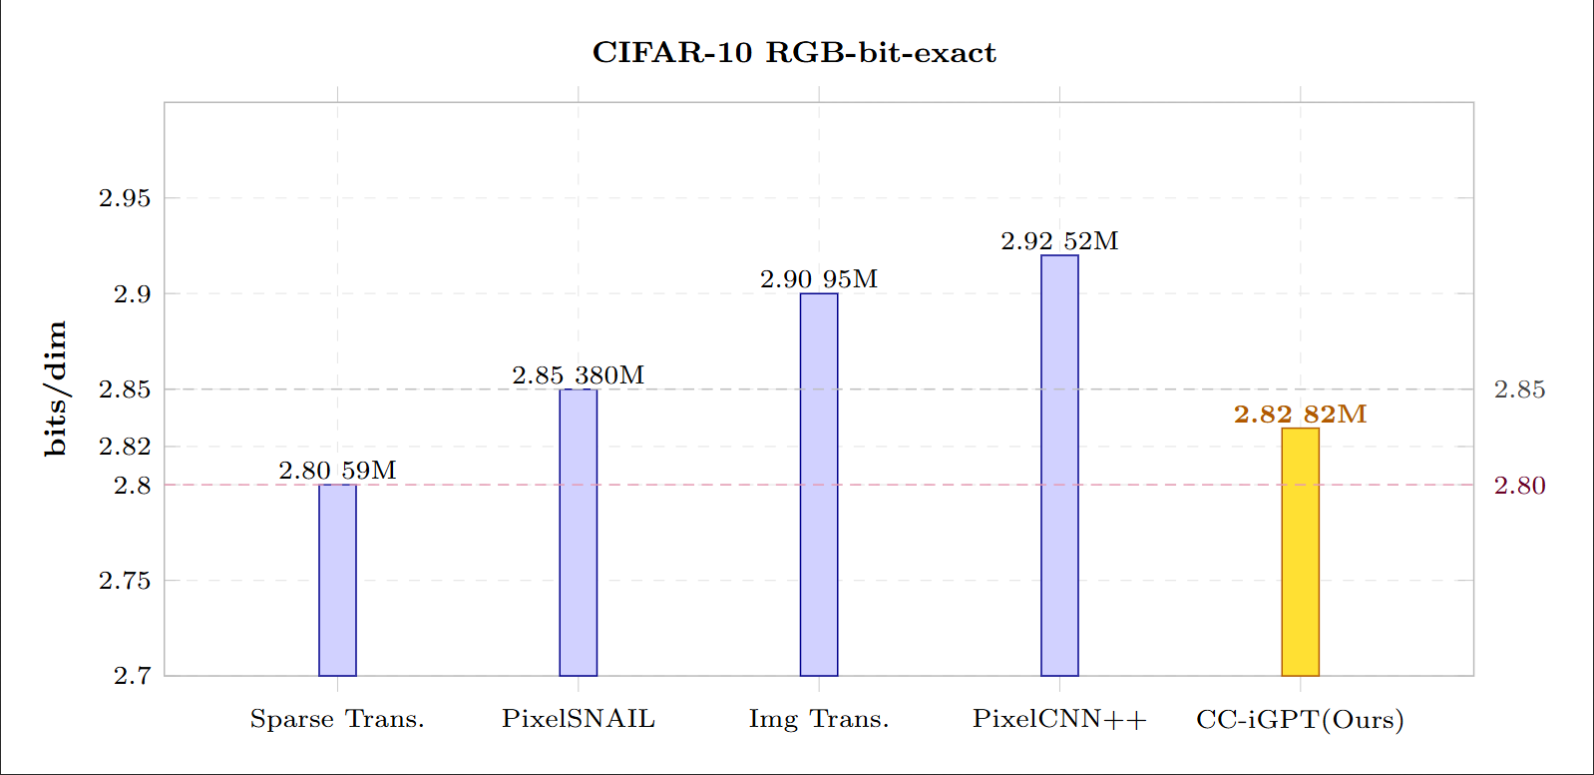
\includegraphics[width=0.92\linewidth]{baseline.png}
\end{center}

\vspace{-2mm}
\centering
\small
\textbf{CC-iGPT v2 R-only}: \alert{\textbf{2.8296}} $\pm$ 0.0854 bpd \;
(82.95\,M params, 200 ep, ensemble + TTA hflip)

\smallskip
{\scriptsize vs PixelSNAIL 380M (2.85) \textbf{$-0.020$} \;\; $\cdot$ \;\; vs Sparse Transformer 59M (2.80) $+0.020$}
\end{frame}

% ============================== 4. 模型架构总览（图） ==============================
\begin{frame}{模型架构：CC-iGPT 双尺度条件 AR}
\begin{center}
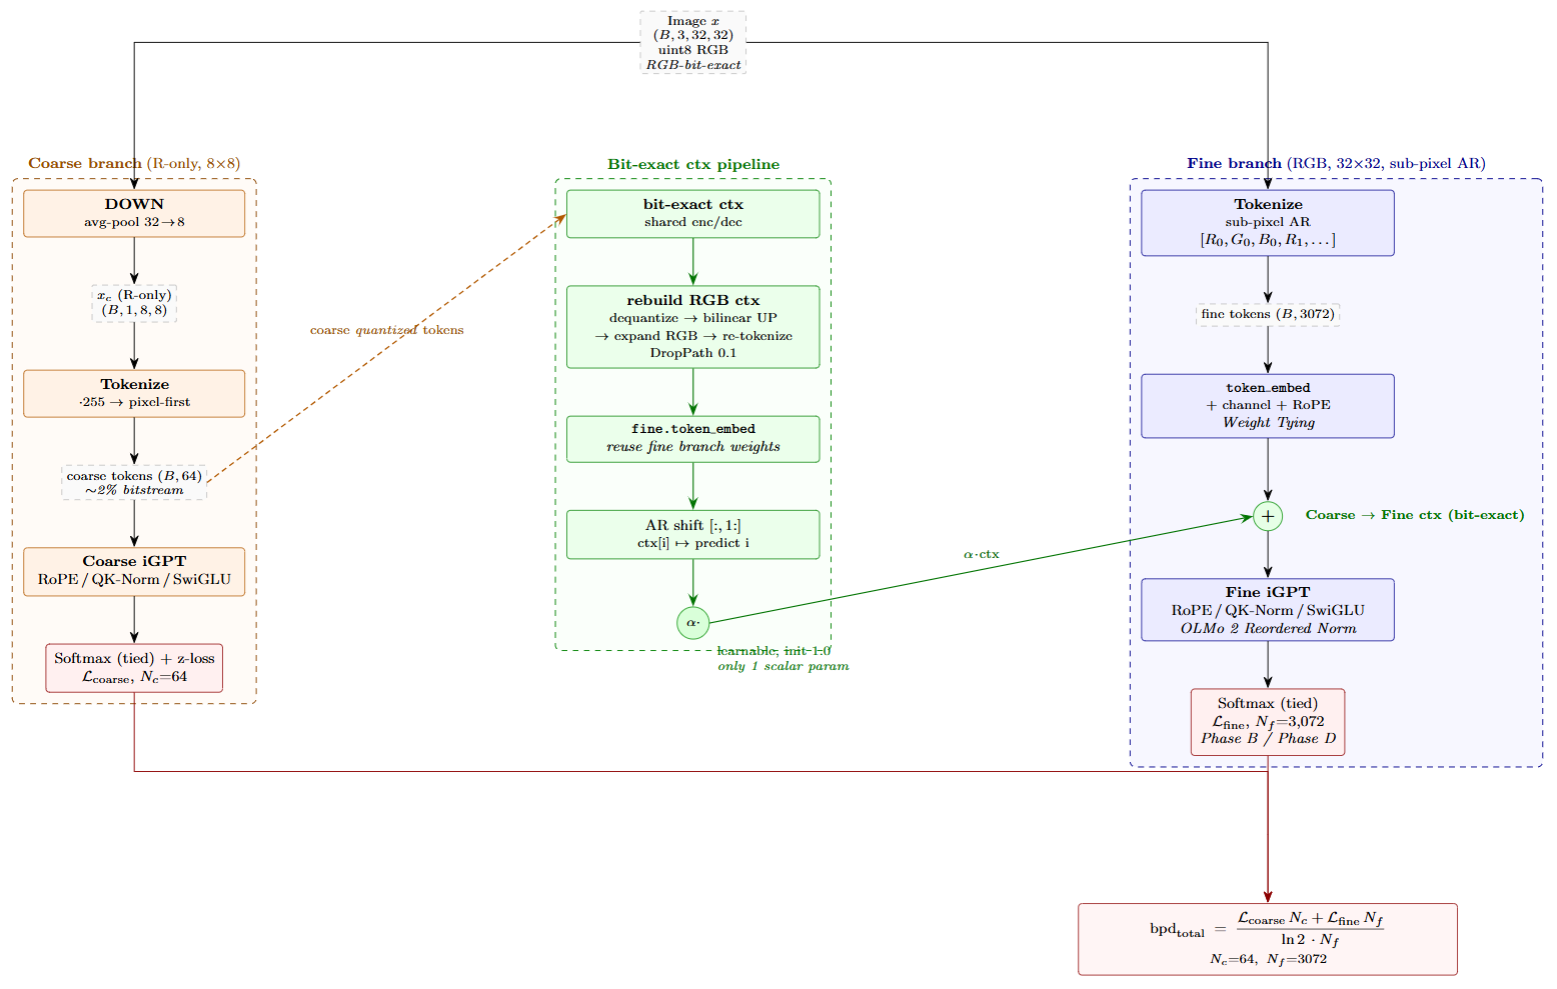
\includegraphics[height=0.78\textheight,keepaspectratio]{cc-igpt_arch.pdf}
\end{center}
\end{frame}

% ============================== 4b. 模型架构（文字） ==============================
\begin{frame}{模型架构：双尺度分解与联合训练}
\begin{columns}[T]
\begin{column}{0.48\textwidth}
\textbf{双尺度分解}
\begin{itemize}
  \item \textbf{Coarse}: DOWN $8{\times}8$ R-only \\
        $\Rightarrow$ 64 token, $\sim$2\% 预算
  \item \textbf{Fine}: $32{\times}32{\times}3$ sub-pixel AR \\
        $\Rightarrow$ 3072 token
\end{itemize}

\bigskip
\textbf{端到端联合训练}
\[
\mathcal{L} = \mathcal{L}_{\text{coarse}} + \mathcal{L}_{\text{fine}}
\]
无尺度间加权，回避多尺度 loss 平衡难题
\end{column}
\begin{column}{0.50\textwidth}
\textbf{联合 bits/dim}
\[
\mathrm{bpd}_{\text{total}} \;=\; \frac{\mathrm{CE}_c\,N_c + \mathrm{CE}_f\,N_f}{\ln 2 \cdot N_f}
\]

\medskip
其中 $N_c = 64$ (coarse 8$\times$8 R), $N_f = 3072$ ($32{\times}32{\times}3$)。

\medskip
\textbf{实测分解（CIFAR-10 主表）}
\begin{itemize}
  \item $\mathrm{CE}_c = 4.3302$ \quad bpd 占比 \alert{4.6\%}
  \item $\mathrm{CE}_f = 1.8711$ \quad bpd 占比 \alert{95.4\%}
  \item $\Rightarrow$ \alert{\textbf{2.8296}} bpd
\end{itemize}
\end{column}
\end{columns}
\end{frame}

% ============================== 5. Coarse pipeline (图) ==============================
\begin{frame}{Coarse GPT pipeline —— $\sim$2\% 预算的「轮廓码」}
\begin{center}
\includegraphics[height=0.78\textheight,keepaspectratio]{Coarse branch pipeline.pdf}
\end{center}
\end{frame}

% ============================== 5b. Coarse pipeline (文字) ==============================
\begin{frame}{Coarse 分支：模块组成与产出}
\begin{columns}[T]
\begin{column}{0.48\textwidth}
\textbf{下采样}
\begin{itemize}
  \item \texttt{F.adaptive\_avg\_pool2d(x, 8)} \\
        float 域 $32 \to 8$
  \item 取 R 通道 $\Rightarrow$ $8{\times}8{\times}1 = 64$ token
\end{itemize}

\bigskip
\textbf{Coarse iGPT（浅层）}
\begin{itemize}
  \item $d_{\text{model}} = 256$, $N = 6$ 层
  \item 标准 NTP 训练
  \item Weight Tying, RoPE, QK-Norm
\end{itemize}
\end{column}
\begin{column}{0.50\textwidth}
\textbf{产出与定位}
\begin{itemize}
  \item $\mathrm{CE}_c = \alert{4.3302}$ \\
        $\Rightarrow$ 直接进 bitstream
  \item bpd 占比仅 \alert{4.6\%}（$\sim$2\% 预算）
  \item 量化 token 作为 \textbf{ctx 桥梁} \\
        交给 fine 分支条件化
\end{itemize}

\bigskip
\textbf{设计动机}
\begin{itemize}
  \item 用极少 bit 编码全局轮廓
  \item 让 fine 端聚焦高频细节
  \item 类比 Laplacian Pyramid (1983)
\end{itemize}
\end{column}
\end{columns}
\end{frame}

% ============================== 6. Fine pipeline (图) ==============================
\begin{frame}{Fine GPT pipeline —— 主压缩主体（占 95.4\% bpd）}
\begin{center}
\includegraphics[height=0.78\textheight,keepaspectratio]{Fine branch pipeline.pdf}
\end{center}
\end{frame}

% ============================== 6b. Fine pipeline (文字) ==============================
\begin{frame}{Fine 分支：Ctx 注入与子像素 AR}
\begin{columns}[T]
\begin{column}{0.48\textwidth}
\textbf{Ctx 注入}
\begin{itemize}
  \item coarse 量化 token \\
        $\to$ bit-exact ctx
  \item $\alpha \cdot \mathrm{ctx}$ \emph{additive} 入口
  \item $\alpha = \alert{0.1009}$（实测）\\
        \scriptsize 模型自适应注入强度
\end{itemize}

\bigskip
\textbf{Fine iGPT（深窄）}
\begin{itemize}
  \item $d_{\text{model}} = 448$, $N = 32$ 层 \\
        (\textbf{82.95\,M} params)
  \item Flash Attn v2, SwiGLU, \\
        RoPE, RMSNorm (post-norm)
\end{itemize}
\end{column}
\begin{column}{0.50\textwidth}
\textbf{子像素 AR 序列}
\[
[R_0,\, G_0,\, B_0,\; R_1,\, G_1,\, B_1,\; \dots]
\]
Causal mask 自然实现
\[
p(G \mid R), \quad p(B \mid R, G)
\]
通道间条件依赖无需额外参数。

\bigskip
\textbf{产出}
\begin{itemize}
  \item $\mathrm{CE}_f = \alert{1.8711}$
  \item bpd 占比 \alert{95.4\%}（主压缩主体）
\end{itemize}
\end{column}
\end{columns}
\end{frame}

% ============================== 7. Bit-exact ctx (图) ==============================
\begin{frame}{Bit-exact ctx pipeline}
\begin{center}
\includegraphics[height=0.78\textheight,keepaspectratio]{bit-exact ctx pipeline.pdf}
\end{center}
\end{frame}

% ============================== 7b. Bit-exact ctx (文字) ==============================
\begin{frame}{Bit-exact ctx pipeline：可解码的条件注入}
\textbf{Pipeline}
\begin{center}
\small
\texttt{coarse 量化 token} $\to$ \texttt{/255 反量化} $\to$ \texttt{bilinear UP $32{\times}32$}
$\to$ \texttt{re-tokenize} $\to$ \texttt{fine.token\_embed} $\to$ \texttt{AR shift [:, 1:]} $\to$ $\alpha\cdot$\texttt{ctx}
\end{center}

\medskip
\begin{itemize}
  \item \textbf{Encoder / decoder 共用同一函数} —— bitstream 真实可解，不是「训练时 oracle」
  \item \textbf{整条 ctx 通路仅引入 1 个标量参数 $\alpha$} —— 零新参注入，避开多尺度联合 AR 的 loss 平衡难题
  \item 复用 \texttt{fine.token\_embed} 完成 ctx 编码 —— 与下游 token 共享语义空间
  \item AR shift \texttt{[:, 1:]} —— ctx[i] 对应 fine 被预测位置 $i$（PixelCNN++ conditional 标准语义）
\end{itemize}
\end{frame}

% ============================== 7c. 编码/解码数据流程图 ==============================
\begin{frame}{Codec 数据流：编码 / 解码对称性}
\begin{center}
\includegraphics[height=0.78\textheight,keepaspectratio]{CC-iGPT codec dataflow.pdf}
\end{center}
\end{frame}

% ============================== 7d. Codec 文字说明 ==============================
\begin{frame}{Codec 数据流：encoder / decoder 同管线}
\begin{columns}[T]
\begin{column}{0.48\textwidth}
\textbf{Encoder（压缩端）}
\begin{enumerate}
  \item DOWN: $x \to x_c$ (R 8$\times$8)
  \item Coarse iGPT $\to$ 概率 $p_c$ \\
        $\Rightarrow$ 算术编码进 bitstream
  \item $x_c$ $\to$ \textbf{ctx pipeline}
  \item Fine iGPT(\,$x_f$ \,$|$ $\alpha\cdot$ctx) \\
        $\Rightarrow$ 概率 $p_f$ \\
        $\Rightarrow$ 算术编码进 bitstream
\end{enumerate}
\end{column}
\begin{column}{0.50\textwidth}
\textbf{Decoder（解压端）}
\begin{enumerate}
  \item 算术解码 coarse token $\hat{x}_c$
  \item $\hat{x}_c$ $\to$ \textbf{同一 ctx pipeline} \\
        {\scriptsize（bit-exact，与 encoder 完全一致）}
  \item Fine iGPT(\,$\cdot$ $|$ $\alpha\cdot$ctx) \\
        逐 token AR 解码 $\hat{x}_f$
  \item 还原 RGB $\hat{x} = x$
\end{enumerate}

\bigskip
\centering
\alert{\textbf{无损 \quad bit-exact \quad 真实可解}}
\end{column}
\end{columns}
\end{frame}

% ============================== 8. 训练 (图) ==============================
\begin{frame}{训练动力学：CC-iGPT v2 R-only training curve}
\begin{center}
\includegraphics[height=0.78\textheight,keepaspectratio]{CC-iGPT R-only training curves.pdf}
\end{center}
\end{frame}

% ============================== 8b. 训练 + Ensemble (文字) ==============================
\begin{frame}{训练 + Ensemble (Phase D, 2026-05-27)}
\begin{columns}[T]
\begin{column}{0.48\textwidth}
\textbf{深窄 + 长程训练}
\begin{itemize}
  \item $N = 32$ / $d = 448$ \\
        (\textbf{82.95\,M} params)
  \item 200 epoch, warmup 5 ep
  \item \texttt{min\_lr\_ratio = 0.05} \\
        {\scriptsize 末段 LR 下限避免 SWA「假平均」}
\end{itemize}

\bigskip
\textbf{平均权重}
\begin{itemize}
  \item EMA 0.9998
  \item SWA last 31 ckpts (start ep170)
\end{itemize}
\end{column}
\begin{column}{0.50\textwidth}
\textbf{In-training landmark}
\begin{itemize}
  \item best ep196: 2.8312
  \item SWA: 2.8276
  \item EMA: 2.8301
\end{itemize}

\bigskip
\textbf{Ensemble + TTA}
\begin{itemize}
  \item logit 域平均（best + SWA + EMA）
  \item TTA hflip 推理增广
\end{itemize}

\end{column}
\end{columns}
\end{frame}

% ============================== 9. Triton Kernel (图) ==============================
\begin{frame}{工程：8 个手写 Triton Kernel —— Speedup}
\begin{center}
\includegraphics[height=0.78\textheight,keepaspectratio]{Triton-kernel-speedup-bar-chart.pdf}
\end{center}
\end{frame}

% ============================== 9b. Triton Kernel (文字) ==============================
\begin{frame}{工程：Kernel 清单与反面案例}
\begin{columns}[T]
\begin{column}{0.50\textwidth}
\textbf{7 个进入训练栈}
\begin{itemize}\setlength{\itemsep}{2pt}
  \item Flash Attention v2 ($\sim$960 行)
  \item Fused CE + z-loss
  \item Fused RMSNorm
  \item Fused Add + RMSNorm
  \item Fused SwiGLU
  \item Fused RoPE
  \item Fused Attn + RoPE
\end{itemize}

\bigskip
约 \textbf{2{,}400 行} Triton 代码，全部手写
\end{column}
\begin{column}{0.48\textwidth}
\textbf{1 个反面案例}
\begin{itemize}
  \item \texttt{fused\_linear\_ce}
  \item $V = 256$ 下 roofline 分析 \\
        $\Rightarrow$ compute-bound \\
        $\Rightarrow$ 失去 cuBLAS GEMM 利用率
  \item 实测比 PyTorch 基线慢 \\
        \alert{保留作工程严谨性证据}
\end{itemize}

\bigskip
\textbf{决策原则}
\begin{itemize}
  \item 不是「写了就保留」
  \item Roofline + 实测双验证
  \item 负收益的 kernel 也是结论
\end{itemize}
\end{column}
\end{columns}
\end{frame}

% ============================== 10. Probe + 总结 ==============================
\begin{frame}{Linear Probe \& 总结}
\begin{columns}[T]
\begin{column}{0.42\textwidth}
\small
\textbf{Linear Probe}（CIFAR-10 表征质量）

\smallskip
\begin{itemize}
  \item CC-iGPT v2 fine + $\alpha\cdot$ctx \\
        best L19 = \alert{\textbf{79.33\%}}
  \item iGPT-S baseline \\
        best L22 = 66.93\%
  \item \textbf{+12.4\,pp} —— ctx 注入显著提升中层表征
\end{itemize}
\end{column}
\begin{column}{0.56\textwidth}
\small
\textbf{三大创新}

\smallskip
\textbf{① 方法} —— 零新参的双尺度条件注入 \\
{\scriptsize coarse 量化 token $\to$ bit-exact ctx $\to$ $\alpha\cdot$additive，仅 1 个标量参数}

\smallskip
\textbf{② 工程} —— 8 个手写 Triton kernel \\
{\scriptsize 7 进入训练栈 + 1 反面案例（V=256 roofline 证伪）}

\smallskip
\textbf{③ 分析} —— RGB-bit-exact 主表 \\
{\scriptsize CIFAR-10 \alert{\textbf{2.8296}} 超越 PixelSNAIL 380M (2.85)，逼近 Sparse Transformer 59M (2.80)，参数预算 82.95M}
\end{column}
\end{columns}

\vfill
\centering
\Large \color{ours} 感谢聆听，敬请批评指正
\end{frame}

\end{document}
